% !Mode:: "TeX:UTF-8"

\chapter{红外无人机目标检测算法轻量化}

\section{引言}
对于实际的红外无人机目标检测任务,任务环境常常是野外开阔地带,因此
检测算法常常需要在移动设备上运行,而对于移动端嵌入式设备,硬件的运算能力和成本都十分有限,因此对算法的内存占用和运行时间有更高的要求。也就是在保证检测精度的同时也要保证实时性,这就需要对算法进行一定程度的轻量化,降低算法的内存占用和运行时间,使得移动端设备也可以实时实现红外无人机目标检测。
本章将在上文提到的算法基础上,应用ghost模块对算法模型进行轻量化,并且在PC端和移动端NVIDIA AGX XAVIER设备上进行算法的性能测试,并对实验结果进行分析。

\section{神经网络模型轻量化}
目前,计算机视觉任务采用的神经网络模型已经从8层发展到100层甚至更多层。从一个大型网络开始训练往往能取得更好的性能,因为大型网络往往可以在原本的高精确度表现下降不多的同时适当地减少冗余参数,相比一开始就训练一个较小的网络,训练大型网络再进行轻量化往往能在目标检测精度和参数量上取得更好的平衡。

\subsection{模型剪枝}
来自基于量化和模型兼职的卷积神经网络压缩算法
卷积神经网络模型剪枝方法分为结构化和非结构化
剪枝。结构化是修剪整个过滤器,非结构化剪枝则是直接
对每层参数进行单独剪枝。为了解决卷积神经网络模型
占用空间和计算量过大的问题,不少研究者想通过对神经
网络进行剪枝以 尽 可 能 地 压 缩 体 积 、提 升 速 度 。 早 期 ,
Hassibi[12]利用二阶泰勒展开选择参数并进行剪枝,以改善
训练和泛化能力;Han 等[13]通过权值大小确定修剪训练后
网络中的不重要连接,以减少网络所需参数;CP 算法采用
LASSO 回归方式选择剪枝通道并进行逐层剪枝[14];SFP 采
用动态剪枝方法,主要依靠权重的范数,保留 BN 层的偏置
系数[15]。上述剪枝方法中都出现了剪枝后模型精度下降
的问题,使得模型在剪枝后的识别效果不佳。

目前,针对卷积神经网络的剪枝方法主要分为两种:
权值剪枝和滤波器剪枝。两个方法都是针对卷积层中的
卷积通道进行剪枝,但判定方法不同,一个是通过权值判
定,另一个是通过滤波器判定。网络模型优化通常是针对
模型占用空间大小、模型识别准确率、模型识别速度 3 个目
标。在目前图形识别的 CNN 网络剪枝方法中,最为典型的
是将 CNN 网络 BN 层中的 γ 参数作为网络剪枝的缩放因
子[16]。由于 BN 层具有加速训练和有效减少过拟合现象的
作用,因此已经被大部分常用的图像识别卷积神经网络模
型所使用。在引入缩放因子 γ 之后,通过对每个卷积通道
后特征图的特征值 γ 进行排序,然后根据排序结果设定剪
枝的阈值。即当前通道特征图的 γ 参数小于该阈值,则对
当前特征图对应的卷积核进行剪枝处理。缩放因子扮演
的是通道选择的角色,缩放因子的正则项和权重损失函数
联合优化,网络自动鉴别不重要的通道并将其移除掉,几
乎不影响网络的泛化性能。这样可以人为设定对整个卷
积神经网络模型的剪枝幅度。例如,设定的阈值在所有卷
积核的所有阈值中排列第 60%,则可以减掉 60% 卷积核
只保留 γ 参数大于 60% 的特征图所对应的卷积核。对于不
同的图像识别和不同的神经网络模型,阈值设定会有很大
区别。然而,这种全局阈值设定方法有一定的局限性。当
剪枝百分比数值设定过小,则节省资源非常有限,剪枝效
果不佳;当剪枝百分比数值设定过大,则会出现准确率大
幅度下降的现象,这种准确率的损失无法通过后期微调加
以恢复。

\subsection{参数量化}
在神经网络模型压缩加速方法中,可以通过对参数的量化
压 缩 参 数 量 ,并 达 到 加 速 神 经 网 络 、减 少 计 算 成 本 的 目
的[17]。然而在量化过程中参数的压缩会导致准确率下降。
为了减少参数量化带来的准确率损失,Han 等[13]提出了一
种共享权重和通过权重进行索引编码以减小权重数量和
存储空间的方法。该方法是指定一系列权值,然后将这些
权值进行数值共享,最后所有的权值都只能从指定的权值
中进行选择,而这些指定的权值则通过 K-means 聚类初始
化质心。K-means 质心的初值对最终结果影响较大,通过
实验对比最终选择均匀量化方法完成质心初始化。均匀
量化的结果输出是通过所有权值的最大值和最小值之间
的均匀间隔实现。确定质心之后再确定量化阈值,一个权
值簇里的所有权值都由这个质心代替,最后对质心进行微
调以恢复精度。参数量化之后对于神经网络的压缩有一
定效果,但是在量化质心的确定方法上仍有不适用的网
络。一些神经网络模型可能更适合按密度量化,比如识别
目标单一的神经网络[18]。该方法只对卷积神经网络中的
参数量化方法进行了优化,因此在选择最优阈值的方法中
还有一定的优化空间。

\subsection{知识蒸馏}
高性能的深度学习网络通常是计算型和参数密集型的,难以应用于资源受限的边缘设备  为了能够在低
资源设备上运行深度学习模型,需要研发高效的小规模网络。  知识蒸馏是获取高效小规模网络的一种新兴方法,
其主要思想是将学习能力强的复杂教师模型中的“知识”迁移到简单的学生模型中。  同时,它通过神经网络的互
学习、自学习等优化策略和无标签、跨模态等数据资源对模型的性能增强也具有显著的效果。  基于在模型压缩和
模型增强上的优越特性,知识蒸馏已成为深度学习领域的一个研究热点和重点。 

\subsection{改进网络结构}
除了通用的剪枝、量化、知识蒸馏等模型轻量化方法之外,常用的使神经网络更高效的方法是设计新型网络。
常见的轻量网络模型有SqueezeNet、Xception、MobileNet、ShuffleNet等。每种网络都提出了一种或几种特殊结构用来减少模型的参数量或者提升模型的推理速度。

(1)SqueezeNet
SqueezeNet的主要策略是用$1\times1$的卷积代替部分$3\times3$的卷积运算,这使得卷积的参数数量减少了9倍。此外,SqueezeNet还减少了$3\times3$卷积的通道数。一个$3\times3$卷积的计算量是$3\times3 \times M \times N$(其中$M$和$N$分别是输入通道数和输出通道数),作者将$M$和$N$减少来达到减少整个模型的参数量的目的。另外,为了提升网络的精度,SqueezeNet将下采样模块后置。作者认为较大的Feature Map含有更多的信息,因此将下采样往分类层移动。这样的调整会提高模型的精度,同时也会增加计算量。
SqueezeNet的压缩策略是依靠将$1\times1$卷积替换成$3\times3$卷积来达到的,其参数数量是等性能的AlexNet的2.14%。从参数数量上来看,SqueezeNet的目的达到了。SqueezeNet的最大贡献在于其开拓了模型压缩这一方向,之后的一系列文章也就此打开。

同时,SqueezeNet的缺点也很明显:
SqueezeNet的侧重的应用方向是嵌入式环境,目前嵌入式环境主要问题是实时性。SqueezeNet的通过更深的深度置换更少的参数数量虽然能减少网络的参数,但是其丧失了网络的并行能力,测试时间反而会更长,这与目前的主要挑战是背道而驰的;
论文的题目非常标题党,虽然纸面上是减少了50倍的参数,但是问题的主要症结在于AlexNet本身全连接节点过于庞大,50倍参数的减少和SqueezeNet的设计并没有关系,考虑去掉全连接之后3倍参数的减少更为合适。
SqueezeNet得到的模型是5MB左右,0.5MB的模型还要得益于Deep Compression。虽然Deep Compression也是这个团队的文章,但是将0.5这个数列在文章的题目中显然不是很合适。

(2)Xception
深度可分离卷积(Depthwise Separable Convolution)率先是由 Laurent Sifre在其博士论文\cite{sifre2014rigid}中提出。这篇文章主要从Inception\cite{szegedy2015going}的角度出发,探讨了Inception和深度可分离卷积的关系,从一个全新的角度解释了深度可分离卷积。再结合stoa的残差网络\cite{he2016deep},作者提出了一种新型的轻量网络结构Xception。Xception取义自Extreme Inception,表示Xception是一种极端的Inception。

Inception模块是一大类在ImageNet上取得顶尖结果的模型的基本模块,例如GoogLeNet、Inception V2/V3和Inception-ResNet。有别于VGG等传统的网络通过堆叠简单的3*3卷积实现特征提取,Inception模块通过组合$1\times1$卷积,$3\times3$卷积,$5\times5$卷积和pooling等结构,用更少的参数和更少的计算开销可以学习到更丰富的特征表示。
通常,在一组特征图上进行卷积需要三维的卷积核,也即卷积核需要同时学习空间上的相关性和通道间的相关性。将这两种相关性显式地分离开来,是Inception模块的思想之一:Inception模块首先使用$1\times1$的卷积核将特征图的各个通道映射到一个新的空间,在这一过程中学习通道间的相关性;再通过常规的$3\times3$或$5\times5$的卷积核进行卷积,以同时学习空间上的相关性和通道间的相关性。
但此时,通道间的相关性和空间相关性仍旧没有完全分离,也即$3\times3$或$5\times5$的卷积核仍然是多通道输入的,显然,当所有$3\times3$或$5\times5$的卷积都作用在只有一个通道的特征图上时,通道间的相关性和空间上的相关性即达到了完全分离的效果。

(2)MobileNet
MobileNet\cite{howard2017mobilenets}模型是Google针对手机等嵌入式设备提出的一种轻量级的深层神经网络,其使用的核心思想便是depthwise separable convolution(深度可分离卷积)。

MobileNet模型基于深度可分离卷积搭建,这是分解卷积的一种形式,它将标准卷积分解为深度卷积和以$1\times1$卷积构成的逐点卷积。对MobileNet而言,深度卷积针对每个输入通道应用一个卷积核。然后逐点卷积应用$1\times1$卷积来聚合输出。标准卷积将过滤核聚合输入形成一系列输出熔炼成一步。深度可分离卷积分解成两层,一层用于过滤,一层用于聚合。这种分解具有显著减少计算和模型大小的效果。

设标准卷积层的输入维度为$D_{F} \times D_{F} \times M$,输出特征图维度为$D_{F} \times D_{F} \times N$,其中$D_{F}$表示一个正方形输入特征图的宽和高,$M$表示输入通道数,$D_{G}$指的是正方形输出特征图的宽和高,$N$表示输出通道数。设标准卷积核大小为$D_{K} \times D_{K} \times M \times N$,其中$D_{F}$是卷积核的空间维度,$M$表示输入通道数,$N$表示输出通道数,则标准卷积的计算消耗为
\begin{equation}
    D_{K} \cdot D_{K} \cdot M \cdot N \cdot D_{F} \cdot D_{F}
\end{equation}

其中计算成本乘法取决于输入通道的数量$M$、输出通道的数量$N$、内核大小$D_{K} \times D_{K}$和特征图大小 [公式] 。MobileNet模型解决了这些术语中的每一个及其相互作用。首先,它使用深度可分离卷积来打破输出通道数量和内核大小之间的相互作用。

标准的卷积运算具有填充效果,基于卷积核的特征和组合特征以产生新的表征。过滤和组合步骤可以通过使用称为深度可分离卷积的分解卷积为2个步骤,以显著降低计算成本。

深度可分离卷积由两部分组成:深度卷积和逐点卷积。我们使用深度卷积来针对每个通道使用一个卷积核。逐点卷积通过使用 [公式] 卷积来针对深度卷积的输出实现线性变换。MobileNets在两个层中都使用了BN和ReLU。
\section{基于ghost卷积的网络结构轻量化}
Ghost 模块是一种替代传统CNN中的卷积操作并且获得更快速度和更小模型体积的方案。通过对比分析ResNet-50网络第一个残差组(Residual group)输出的特征图可视化结果,发现一些特征图高度相似。如果按照传统的思考方式,可能认为这些相似的特征图存在冗余,是多余信息,想办法避免产生这些高度相似的特征图。而ghost模块另辟蹊径,选择以一种更简单的操作来生成相同数量的特征图,从而实现更快速高效的检测。

\subsection{Ghost模块思想}
典型的卷积计算过程如图\ref{conv}所示,所有的输入逐一经过卷积运算后生成新的特征图。这里的每一个输出张量都是一个由卷积核运算产生的特征图。但是这些特征图中可能有些特征图相似度较高,因此可以认为两张或几张比较相似的特征图是产生于几次同样代价的卷积是一种浪费。

\begin{figure}[htbp]
    \centering
    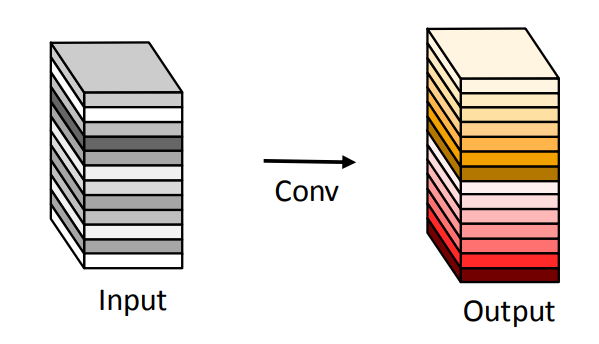
\includegraphics[width = 0.5\textwidth]{传统卷积.png}
    \caption{传统卷积示意图}
    \label{conv}
\end{figure}

如图\ref{identical}所示,每次卷积的所有输出中,可以找到一些相互之间相似度较高的特征图。设图中的A, A’、B B’相似度较高,可以设计一种计算方法替代生成A’和B’的卷积运算,从而达到减小计算量的目的。

\begin{figure}[htbp]
    \centering
    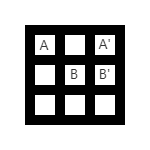
\includegraphics[width = 0.5\textwidth]{重复特征图.png}
    \caption{重复特征图示意图}
    \label{identical}
\end{figure}

\begin{figure}[htbp]
    \centering
    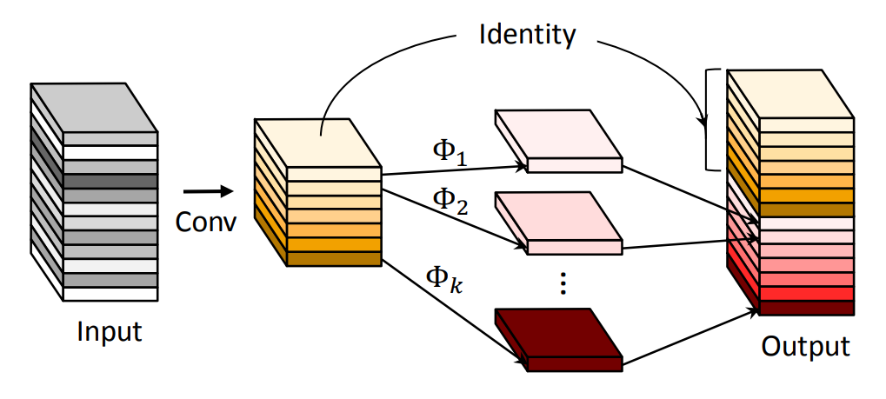
\includegraphics[width = 0.5\textwidth]{ghost卷积.png}
    \caption{ghost卷积示意图}
    \label{ghost1}
\end{figure}

如图\ref{ghost1}所示,ghost模块的做法是用一些更小的卷积核(即参数更少运算更快)替代原先的卷积部分,但是这部分卷积核产生的输出量只能达到相当于本来卷积输出量的一部分,这时根据上文对相似特征图的分析,可以采用一些线性变换的方式去生成剩下的特征图,从而达到用更轻量的卷积滤波器去生成相同规模特征图的目的。

\subsection{基于ghost模块的模型轻量化算法实现}

\begin{figure}[htbp]
    \centering
    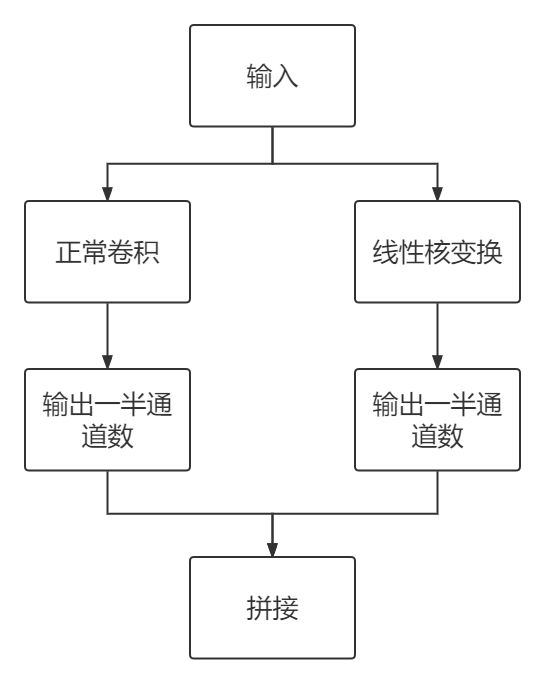
\includegraphics[width = 0.6\textwidth]{ghost算法实现.png}
    \caption{ghost算法实现示意图}
    \label{ghost2}
\end{figure}

本课题的Ghost实现流程如图\ref{ghost2}所示,将原始卷积层改变成两部分,分别产生相当于原始卷积层一半通道数的输出(实际上二者的输出比例可以任意调节),可以使得改进后的模块参数量减少。

\begin{figure}[htbp]
	\centering
	\begin{minipage}{0.49\linewidth}
		\centering
		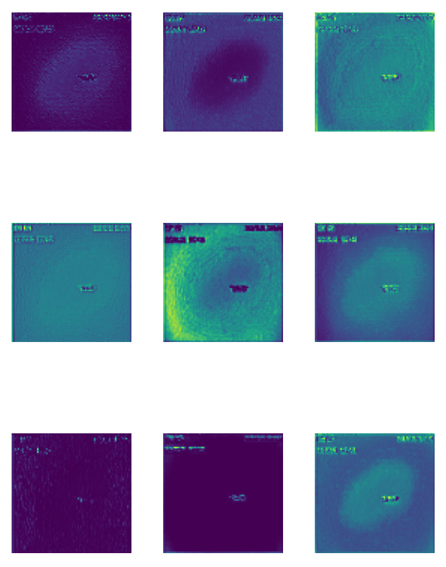
\includegraphics[width=0.9\linewidth]{convfmap.PNG}
		\caption{普通卷积特征图}
		\label{convf}%文中引用该图片代号
	\end{minipage}
	%\qquad
	\begin{minipage}{0.49\linewidth}
		\centering
		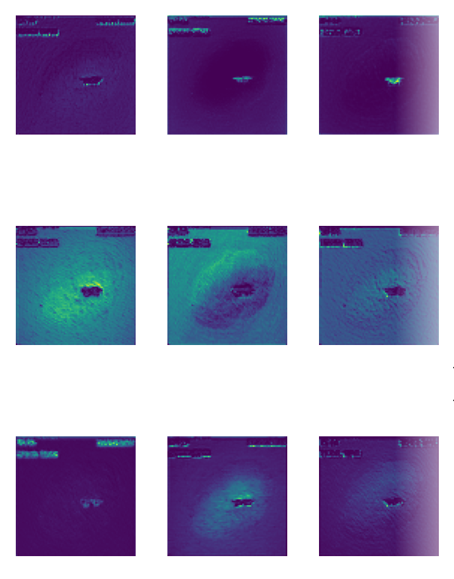
\includegraphics[width=0.9\linewidth]{ghostfmap.PNG}
		\caption{ghost卷积特征图}
		\label{ghostf}%文中引用该图片代号
	\end{minipage}
\end{figure}

普通卷积和ghost卷积产生的特征图如图\ref{convf}和图\ref{ghostf}所示,从图中可以看出,由于ghost卷积相当于对普通卷积进行了一定程度的转化,所以ghost卷积产生的特征图和普通卷积产生的特征图存在一定的差别,不过图\ref{convf}和图\ref{ghostf}中确实有相当大比例的对应位置特征图是相似的,这也验证了上文的理论分析。此外,由于ghost卷积减少了网络结构中的参数,所以在简化运算、加速推理的同时,各特征图之间的差异更小,也就是ghost卷积产生的特征图在一定程度上丢失了多样性,也将导致整个网络失去一些特征,降低最终目标检测的精度。

\subsection{ghost算法理论分析}
对于特定的网络结构,在将传统卷积模块替换成ghost卷积模块之后,可以对网络模型的参数数量和推理速度进行理论计算,得出改进后网络相对于原网络的推理加速比和参数压缩比。

(1)相对于普通卷积模块的加速比

\begin{equation}
    \begin{aligned}
    r_{s} &=\frac{n \cdot h^{\prime} \cdot w^{\prime} \cdot c \cdot k \cdot k}{\frac{n}{s} \cdot h^{\prime} \cdot w^{\prime} \cdot c \cdot k \cdot k+(s-1) \cdot \frac{n}{s} \cdot h^{\prime} \cdot w^{\prime} \cdot d \cdot d} \\
    &=\frac{c \cdot k \cdot k}{\frac{1}{s} \cdot c \cdot k \cdot k+\frac{s-1}{s} \cdot d \cdot d} \approx \frac{s \cdot c}{s+c-1} \approx S
    \end{aligned}
    \label{jsb}
\end{equation}

如式\ref{jsb}所示,设输入通道数为$c$,输出通道数为$n$,输入图像高度为$h^{\prime}$和$w^{\prime}$,其中保留的原始卷积通道数为本来的$1/s$,原始卷积核大小为$k*k$,线性核大小为$d*d$,由于线性变换是在每个通道上进行,所以代表线性变换的一项中不含输入通道数$c$。

由式\ref{jsb}可得,将原始卷积模块替换为一半卷积一半线性变换的ghost模块后(即将$s=2$代入),可以得到该模块的理论提速比为2。

(1)相对于普通卷积模块的参数压缩比

\begin{equation}
    r_{c}=\frac{n \cdot c \cdot k \cdot k}{\frac{n}{s} \cdot c \cdot k \cdot k+(s-1) \cdot \frac{n}{s} \cdot d \cdot d} \approx \frac{s \cdot c}{s+c-1} \approx \frac{s c}{c}=S
    \label{csys}
\end{equation}

如式\ref{csys}所示,经过计算可以得到改进后的ghost模块和改进之前的普通卷积模块理论参数压缩比为2。

\subsection{ghost算法实验对比分析}
将ghost模块对应改动部署到YOLOv5网络之后,在实验平台上进行测试验证。分别用YOLOv5网络模型和调整深度之后得到的小型网络(记为YOLOv5s)作为参照,验证YOLOv5+ghost在红外无人机图像数据集上的效果。

\section{轻量化红外无人机目标检测算法嵌入式实现与验证}
为了进一步验证本文提出的轻量化红外无人机目标检测算法的有效性,本节将本文提出的完整算法模型进行转换,并且在嵌入式设备上进行检测和验证。

\subsection{嵌入式设备介绍}
为了满足实际检测任务的需要,本章将本文提到的算法在常用于深度的嵌入式设备 NVIDIA
Jetson AGX Xavier 上进行算法测试,验证算法在实际使用中是否能达到实时性要求。
NVIDIA Jetson AGX Xavier 开发板是英伟达公司推出的嵌入式 AI 超级计算平台,可以
部署在无人机或机器人等诸多终端上,解决移动终端算力不足的局限。NVIDIA
Jetson TX2 采用 Tegra 处理器,内存为 8GB,采用了全新 Pascal 架构 GPU 核心,
更加适合进行一些基于深度学习的计算机视觉任务的开发,具体参数如表\ref{t1}中所
示。NVIDIA Jetson AGX Xavier 具有 MAX Q 和 MAX P 两种运行模式,由于其体型小巧,
性能高效,因此应用场景广泛,如无人机和智能机器人等相关的智能机器领域,
安防和智慧城市等领域。NVIDIA Jetson AGX Xavier 平台出厂自带 Ubuntu 16.04 操作系
统,支持 NVIDIA Jetpack SDK,包括深度学习库、计算机视觉、GPU 计算等功
能,支持下载安装所有台式机所能安装的软件如 Python、Pytorch、TensorFlow
等,轻松配置台式机一样的运行环境。NVIDIA Jetson AGX Xavier 有非常多功能的接口,
比如可以使用 HDMI 接口连接显示器,使用 USB3.0 接口连接摄像头进行实时获
取视频数据用来进行检测或跟踪任务。NVIDIA Jetson AGX Xavier 嵌入式开发平台如图
5.1 所示。近年来由于 TX2 嵌入式平台外形小巧便于集成到各种终端产品中,嵌
入式智能计算平台发展迅猛,但经过实际测试表明嵌入式设备因为 CPU 和 GPU
计算能力与台式机相比仍具有一定差距,TX2 与台式机在相同参数情况下进行相
同的实验时,二者 GPU 运算效率相差将近 10 倍。由于人工智能的兴起,未来嵌
入式设备会向着更加小型化、功耗更低、运行速度更快的方向发展。

\begin{table}[htbp]
    \caption{不同算法对红外无人机数据集的检测结果}
    \vspace{0.5em}\centering\wuhao
    \begin{tabular}{cc}
    \toprule
    项目 & 规格\\
    \midrule
    GPU & 512核 NVIDIA Volta GPU,64 Tensor核\\
    CPU & 8核 ARM v8.2 64-bit CPU, 8MB L2 + 4MB L3\\
    DL Accelerator & 2x NVDLA\\
    Vision Accelerator & 2x PVA\\
    Memory & 32GB 256-bit LPDDR4x\\
    Storage & 32GB eMMC 5.1\\
    CSI Camera & 16 lanes MIPI CSI-2\\
    PCIe & x16 connector with x8 PCIe Gen4 or x8 SLVS-EC\\
    Networking & RJ45 (Gigabit Ethernet)\\
    尺寸 & 105mm x 105mm x 65mm\\
    \bottomrule
    \end{tabular}
    \label{t1}
\end{table}

\subsection{tensorrt加速}
% https://github.com/wang-xinyu/tensorrtx/blob/master/tutorials/from_pytorch_to_trt_stepbystep_hrnet.md

\subsection{不同算法性能对比与分析}


